\documentclass{article}
\usepackage{amsmath,amssymb,graphicx,subfig,mathrsfs,amsthm}
\newcommand{\inner}[2]{\langle #1, #2 \rangle}
\newcommand{\Res}{\textrm{Res}} 
\newcommand{\SO}{\textrm{SO}} 
\newcommand{\Diff}{\textrm{Diff}} 
\newcommand{\Sympl}{\textrm{Sympl}} 
\newcommand{\Lie}{\textrm{Lie}} 
\newcommand{\id}{\textrm{id}} 
\newcommand{\Ad}{\textrm{Ad}} 
\newcommand{\norm}[1]{\left\Vert #1 \right\Vert}
\newtheorem{theorem}{Theorem}
\newtheorem{lemma}[theorem]{Lemma}
\newtheorem{corollary}[theorem]{Corollary}
\begin{document}
\title{Hamiltonian flows, cotangent lifts, and momentum maps}
\author{Jordan Bell}
\date{April 3, 2014}

\maketitle

\section{Symplectic manifolds}
Let $(M,\omega)$ and $(N,\eta)$ be symplectic manifolds. A {\em symplectomorphism} $F:M \to N$ is a diffeomorphism
such that $\omega=F^* \eta$. Recall that for $x \in M$ and $v_1,v_2 \in T_xM$,
\[
(F^* \eta)_x(v_1,v_2)=\eta_{F(x)}((T_x F)v_1,(T_x F)v_2);
\]
$T_x F: T_x M \to T_{F(x)}N$. (A tangent vector at $x \in M$ is {\em pushed forward} to a tangent vector at $F(x) \in N$, while a differential 2-form on $N$ is {\em pulled back} to a 
differential 2-form on $M$.) In these notes the only symplectomorphisms in which we are interested  are those from a symplectic manifold to itself.\footnote{I am interested in flows
on a phase space and this phase space is a symplectic manifold. For some motivation for why we want phase space to be a symplectic manifold, read:

 http://research.microsoft.com/en-us/um/people/cohn/thoughts/symplectic.html}

\section{Symplectic gradient}
If $(M,\omega)$ is a symplectic manifold and $H \in C^\infty(M)$, using the nondegeneracy of the symplectic form $\omega$ one can prove that there is a unique
vector field
$X_H \in \Gamma^\infty(M)$ 
such that, for all $x \in M, v \in T_xM$,
\[
\omega_x(X_H(x),v)=(dH)_x(v).
\]
This can also be written as 
\[
i_{X_H} \omega = dH,
\]
where 
\[
(i_X \omega)(Y)= (X \lrcorner \omega)(Y)=\omega(X,Y).
\]
We call $X_H$ the {\em symplectic gradient} of $H$. If $X \in \Gamma^\infty(M)$ and $X=X_H$ for some $H \in C^\infty(M)$, we say that $X$ is a {\em Hamiltonian vector
field}.\footnote{On a Riemannian manifold, a vector field that is the gradient of a smooth function is called a {\em gradient vector field} or a {\em conservative
vector field}.}

Let's check that 
\[
X_H = \sum_{i=1}^n \frac{\partial H}{\partial p_i} \frac{\partial}{\partial q_i}-\frac{\partial H}{\partial q_i}\frac{\partial}{\partial p_i}.
\]
We have, because $dq_i \frac{\partial}{\partial q_j}=\delta_{ij}$,  $dp_i \frac{\partial}{\partial p_j}=\delta_{ij}$, $dq_i \frac{\partial}{\partial p_j}=0$
and $dp_i \frac{\partial}{\partial q_j}=0$, and because $dq_j \wedge dp_j = - dp_j \wedge dq_j$,
\begin{eqnarray*}
i_{X_H} \omega&=&\sum_{i=1}^n dq_i \wedge dp_i  \sum_{j=1}^n \left( \frac{\partial H}{\partial p_j} \frac{\partial}{\partial q_j}-\frac{\partial H}{\partial q_j}\frac{\partial}{\partial p_j} \right)\\
&=&\sum_{i=1}^n dq_i \wedge dp_i \left(\frac{\partial H}{\partial p_i} \frac{\partial}{\partial q_i}-\frac{\partial H}{\partial q_i}\frac{\partial}{\partial p_i} \right)\\
&=&\sum_{i=1}^n \frac{\partial H}{\partial p_i} dp_i + \frac{\partial H}{\partial q_i} dq_i\\
&=&dH.
\end{eqnarray*}



\section{Flows}
Let $M$ be a smooth manifold. Let $D$ be an open subset of $M \times \mathbb{R}$, and for each $x \in M$ suppose that
\[
D^x = \{t \in \mathbb{R}: (x,t) \in D\}
\]
is an open interval including $0$. 
A {\em flow} on $M$ is a smooth map $\phi:D \to M$ such that if $x \in M$ then $\phi_0(x)=x$
and such that
if $x \in M$, $s \in D^x, t \in D^{\phi_s(x)}$ and $s+t \in D^x$, then
\[
\phi_t(\phi_s(x))=\phi_{s+t}(x).
\]
For $x \in M$, define $\phi^x:D^x \to M$ by $\phi^x(t)=\phi_t(x)$. 
The {\em infinitesimal generator} of a flow $\phi$ is the vector field $V$  on $M$ defined  for $x \in M$ by
\[
V_x=\frac{d}{dt}\Big|_{t=0} \phi^x(t).
\]
It is a fact that every vector field on $M$ is the infinitesimal generator of a flow on $M$, and furthermore that there is a unique flow whose domain is maximal
that has that vector field as its infinitesimal generator, and we thus speak of {\em the} flow of a vector field.

We say that a vector field is {\em complete} if it is the infinitesimal generator of a flow whose domain is $\mathbb{R} \times M$, in other words if it is the infinitesimal generator
of a {\em global flow}. It is a fact that if $V$ is a vector field on a compact smooth manifold then $V$ is complete.

\section{Hamiltonian flows}
Let $(M,\omega)$ be a symplectic manifold.
We say that a vector field $X$ on $M$ is {\em symplectic} if
\[
\mathcal{L}_X \omega=0,
\]
where $\mathcal{L}_X \omega$ is the Lie derivative of $\omega$ along the flow of $X$. A {\em Hamiltonian flow} is the flow
of a Hamiltonian vector field.\footnote{cf. gradient flow.}
If $X$ is a complete symplectic vector field and $\phi:M \times \mathbb{R}$ is the flow of $X$, then for all $t \in \mathbb{R}$,
the map $\phi_t:M \to M$ is a symplectomorphism.

Let $H \in C^\infty(M)$, and let $\phi$ be the flow of the vector field $X_H$. If $(x,s)$ is in the domain of the flow
$\phi$, we have
\begin{eqnarray*}
\frac{d}{dt}\Big|_{t=s} H(\phi^x(t)) &=&(d_{\phi^x(s)}H)((\phi^x)'(s))\\
&=&(d_{\phi^x(s)}H)(X_H(\phi^x(s)))\\
&=&\omega_{\phi^x(s)}(X_H(\phi^x(s)),X_H(\phi^x(s)))\\
&=&0.
\end{eqnarray*}
Thus a Hamiltonian vector field is symplectic: $H$ does not change along the flow of $X_H$. We can also write this as
\begin{eqnarray*}
\frac{d}{dt} (H \circ \phi_t) &=&\frac{d}{dt}(\phi_t^* H)\\
&=&\phi_t^* (\mathcal{L}_{X_H} H)\\
&=&\phi_t^*((i_{X_H} \omega)(X_H))\\
&=&\phi_t^*(\omega(X_H,X_H))\\
&=&\phi_t^*(0)\\
&=&0.
\end{eqnarray*}

It is a fact that if $H_{\textrm{dR}}^1(M)=\{0\}$ (i.e. if $\alpha$ is a 1-form on $M$ and $d\alpha=0$ then
there is some $f \in C^\infty(M)$ such that $\alpha=df$) then every symplectic vector field on $M$ is Hamiltonian. In particular,
if $M$ is simply connected then $H_{\textrm{dR}}^1(M)=\{0\}$, and hence if $M$ is simply connected then every
symplectic vector field on $M$ is Hamiltonian.

\section{Poisson bracket}
For $f,g \in C^\infty(M)$, we define $\{f,g\} \in C^\infty(M)$ for $x \in M$ by
\[
\{f,g\}(x)=\omega_x(X_f(x),X_g(x)).
\]
This is called the {\em Poisson bracket} of $f$ and $g$.
We write
\[
\{f,g\}=\omega(X_f,X_g).
\]
We have
\[
\{f,g\}=X_f g=(df)X_g.
\]
We say that $f$ and $g$ {\em Poisson commute} if $\{f,g\}=0$. The 
Poisson bracket of $f$ and $g$ tells us how $f$ changes along the Hamiltonian flow of $g$. If $f$ and $g$ Poisson commute
then $f$ does not change along the flow of $X_g$.

We have
\begin{eqnarray*}
\{f,g\}&=&\omega(X_f,X_g)\\
&=&\sum_{i=1}^n (dq_i \wedge dp_i) \sum_{j=1}^n  \left( \frac{\partial f}{\partial p_j} \frac{\partial}{\partial q_j}-\frac{\partial f}{\partial q_j}\frac{\partial}{\partial p_j} \right)
 \sum_{k=1}^n  \left( \frac{\partial g}{\partial p_k} \frac{\partial}{\partial q_k}-\frac{\partial g}{\partial q_k}\frac{\partial}{\partial p_k} \right)\\
 &=&\sum_{i=1}^n  \left( \frac{\partial f}{\partial p_i} dp_i + \frac{\partial f}{\partial q_i} dq_i \right) \sum_{k=1}^n  \left( \frac{\partial g}{\partial p_k} \frac{\partial}{\partial q_k}-\frac{\partial g}{\partial q_k}\frac{\partial}{\partial p_k} \right)\\
 &=&\sum_{i=1}^n -\frac{\partial f}{\partial p_i} \frac{\partial g}{\partial q_i}+\frac{\partial f}{\partial q_i} \frac{\partial g}{\partial p_i}.
\end{eqnarray*}

If $x \in M$ and $v \in T_xM$,  then $vf$ is the directional derivative in the direction $v$. If $v=\sum_{i=1}^n a_i \frac{\partial}{\partial q_i}+b_i \frac{\partial}{\partial p_i}$
and $f \in C^\infty(M)$ then
\[
vf=\sum_{i=1}^n a_i \frac{\partial f}{\partial q_i}+b_i \frac{\partial f}{\partial p_i}.
\]
If $X$ is a vector field on $M$ then $Xf \in C^\infty(M)$, defined for
$x \in M$ by
\[
(Xf)(x)=X_x f.
\]
If $\tau$ is a covariant tensor field and $X$ is a vector field, the Lie derivative of $\tau$ along the flow of $X$ is defined as follows: if $\phi$ is the flow of $X$, then
\[
(\mathcal{L}_X \tau)(x)=\frac{d}{dt}\Big|_{t=0} (\phi_t^* \tau)(x),
\]
and so if $\tau$ is a function $f \in C^\infty(M)$, then
\[
(\mathcal{L}_X f)(x)=\frac{d}{dt}\Big|_{t=0} (\phi_t^* f)(x)=\frac{d}{dt}\Big|_{t=0} f(\phi_t(x))=X_x f = (Xf)(x).
\]
Thus if $X$ is a vector field and $f \in C^\infty(M)$, then $\mathcal{L}_X f=Xf$.

For $f,g\in C^\infty(M)$,
\begin{eqnarray*}
X_{\{f,g\}} \lrcorner \omega&=&d\{f,g\}\\
&=&d(X_g f)\\
&=&d(\mathcal{L}_{X_g} f)\\
&=&\mathcal{L}_{X_g}(df)\\
&=&\mathcal{L}_{X_g}(X_f \lrcorner \omega)\\
&=&(\mathcal{L}_{X_g} X_f)\lrcorner \omega+X_f \lrcorner \mathcal{L}_{X_g}\omega\\
&=&[X_g,X_f]\lrcorner \omega + X_f \lrcorner 0\\
&=&[X_g,X_f]\lrcorner \omega\\
&=&-[X_f,X_g]\lrcorner \omega.
\end{eqnarray*}
Since the symplectic form $\omega$ is nondegenerate, if $X \lrcorner \omega= Y \lrcorner \omega$ then $X=Y$, so
\[
X_{\{f,g\}}=-[X_f,X_g].
\]
It follows that $C^\infty(M)$ is a Lie algebra using the Poisson bracket as the Lie bracket.

The set $\Gamma^\infty(M)$ of vector fields on $M$ are a Lie algebra using the vector field commutator $[\cdot,\cdot]$. The symplectic vector fields
are a Lie subalgebra: it is clear that they are a linear subspace of the Lie algebra of vector fields, and one shows that the commutator
of two symplectic vector fields is itself a symplectic vector field. One can further show that the set of Hamiltonian vector fields is a Lie subalgebra
of the Lie algebra of symplectic vector fields. It is a fact that the vector space quotient of the vector space of symplectic vector fields modulo the vector space
of Hamiltonian vector
fields is isomorphic to the vector space $H_{\textrm{dR}}^1(M)$; this is why if $H_{\textrm{dR}}^1(M)=\{0\}$ (in particular if $M$ is simply connected) then any symplectic vector field on $M$ is Hamiltonian.

\section{Tautological 1-form}
Let $Q$ be a smooth manifold and let $\pi:T^*Q \to Q$, $\pi(q,p)=q$. For $x=(q,p) \in T^*Q$, we have
\[
d_x \pi: T_x T^* Q \to T_q Q.
\]
Let
\[
\theta_x = (d_x \pi)^* (p)=p \circ d_x \pi: T_x T^* Q  \to \mathbb{R}.
\]
Thus $\theta: T^*Q \to T^*T^*Q$.  $\theta$ is called the {\em tautological 1-form} on $T^*Q$. 

If $(Q_1,\ldots,Q_n)$ are coordinates on an open subset $U$ of $Q$, $Q_i:U \to \mathbb{R}$, then for each $q \in U$ we
have that $d_q Q_i \in T_q^*U=T_q^* Q$, $1 \leq i \leq n$, are a basis for $T_q^* Q$ and $\frac{\partial}{\partial Q_i}\big|_q$, $1 \leq i \leq n$, are a basis for $T_qQ$. For each $p \in T_q^* Q$,
\[
p=\sum_{i=1}^n p\left(\frac{\partial}{\partial Q_i}\Big|_q \right) d_q Q_i.
\] 
On $T^*U$, define coordinates $(q_1,\ldots,q_n,p_1,\ldots,p_n)$ by 
\[
q_i(q,p)=Q_i(q),
\]
and
\[
p_i(q,p)=p\left(\frac{\partial}{\partial Q_i}\Big|_q \right).
\]
On $T^*U$ we can
write $\theta$ using these coordinates: for $x=(q,p) \in T^*Q$,
\[
\theta_x = p \circ d_x \pi = \sum_{i=1}^n p_i(x) d_x q_i.
\]
Thus, on $T^*U$,
\[
\theta=\sum_{i=1}^n p_i dq_i.
\]

Let $\omega=-d\theta$. We have, on $T^*U$,
\begin{eqnarray*}
\omega&=&-d \sum_{i=1}^n p_i dq_i\\
&=&-\sum_{i=1}^n \left(dp_i \wedge dq_i +  p_i d(dq_i) \right)\\
&=&-\sum_{i=1}^n dp_i \wedge dq_i\\
&=&\sum_{i=1}^n dq_i \wedge dp_i.
\end{eqnarray*}
$T^*Q$ is a symplectic manifold with the symplectic form $\omega$.

\section{Cotangent lifts}
Let $Q$ be a smooth manifold and let $F:Q \to Q$ be a diffeomorphism. Define
\[
F^\sharp:T^*Q \to T^*Q
\]
for $x=(q,p)$ by
\[
F^\sharp(q,p)=(F(q),(d_{F(q)} (F^{-1}))^*(p)).
\]
We call $F^\sharp:T^*Q \to T^*Q$ the {\em cotangent lift} of $F:Q \to Q$. It is a fact that it is a diffeomorphism. It is apparent that the following diagram commutes:

\begin{figure}
\begin{center}
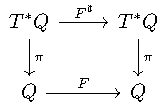
\includegraphics[width=0.4\textwidth]{tikz}
\end{center}
\end{figure}


The pull-back of $\theta$ by $F^\sharp$ satisfies, for $x=(q,p) \in T^*Q$ and $(\zeta,\eta)=F^\sharp(q,p) \in T^*Q$,
\begin{eqnarray*}
((F^\sharp)^* \theta)_x&=&(d_x F^\sharp)^*(\theta_{F^\sharp(x)})\\
&=&(d_x F^\sharp)^* ((d_{F^\sharp(x)} \pi)^*(\eta))\\
&=&(d_x (\pi \circ F^\sharp))^*(\eta)\\
&=&(d_x (F \circ \pi))^* (\eta)\\
&=&(d_x \pi)^* ( (d_{\pi(x)} F)^*(\eta)    )\\
&=&(d_x \pi)^* ( (d_q F)^*(\eta))\\
&=&(d_x \pi)^* (p)\\
&=&\theta_x.
\end{eqnarray*}
Thus $(F\sharp)^*\theta = \theta$, i.e. $F^\sharp$ pulls back $\theta$ to $\theta$. The ``naturality of the exterior derivative''\footnote{For each $k$, $\Omega^k$ is a contravariant functor, and  if $f:M \to N$, then the functor $\Omega^k$ sends $f$ to $f^*:\Omega^k(N) \to \Omega^k(M)$.
$d$ is a natural transformation from the contravariant functor $\Omega^k$ to the contravariant functor $\Omega^{k+1}$.} is the statement
that if $G$ is a smooth map and $\eta$ is a differential form then $G^*(d\eta)=d(G^*\eta)$. Hence, with $\omega=d\theta$,
\[
(F^\sharp)^* \omega = (F^\sharp)^* (d\theta)=d((F^\sharp)^* \theta)=d(\theta)=\omega,
\]
so $F^\sharp$ pulls back the symplectic form $\omega$  to  itself. Thus $F^\sharp:T^*M \to T^*M$ is a symplectomorphism.


Let $\Diff(Q)$ be the set of diffeomorphisms $Q \to Q$. $\Diff(Q)$ is a group. Let $G$ be a group and let $\tau:G \to \Diff(Q)$ be a homomorphism.
Define $\tau^\sharp:G \to \Diff(T^*Q)$ by $(\tau^\sharp)_g=(\tau_g)^\sharp:T^*Q \to T^*Q$. 
$\tau^\sharp:G \to \Diff(T^*Q)$ is a homomorphism, and for each $g \in G$, $(\tau^\sharp)_g:T^*Q \to T^*Q$ is a symplectomorphism.
In words, if a group acts by diffeomorphisms on a smooth manifold, then the cotangent lift of the action is an action by symplectomorphisms
on the cotangent bundle.

\section{Lie groups}
Recall that if
$F:M \to N$ then $TF:TM \to TN$ satisfies, for $X \in \Gamma^\infty(M)$ and $f \in C^\infty(N)$,\footnote{In words: $TF$ pushes forward a vector field on $M$ to a vector field
on $N$.}
\[
((TF) X)(f)=X(f \circ F),
\]
i.e. for $x \in M$ and $v \in T_xM$,
\[
((T_x F) v)(f)=v(f\circ F),
\]
the directional derivative of $f \circ F \in C^\infty(M)$ in the direction of the tangent vector $v$.

Let $G$ be a Lie group and for $g \in G$ define $L_g:G \to G$ by $L_g h=gh$. 
If $X$ is a vector field on $G$, we say that $X$ is {\em left-invariant} if 
\[
(T_h L_g)(X_h)=X_{gh}
\]
for all $g,h \in G$. That is, $X$ is left-invariant if 
\[
(T L_g)(X)=X
\]
for all $g \in G$. 

If $X$ and $Y$ are left-invariant vector fields on $G$ then so is $[X,Y]$. This is because, for $F:G \to G$,
\[
(TF)[X,Y]=[(TF)X,(TF)Y].
\]
Thus the set of left-invariant vector fields on $G$ is a Lie subalgebra of the Lie algebra of vector fields on $G$.

Define $\epsilon:\Lie(G) \to T_e G$ by $\epsilon(X)=X_e$, where $e \in G$ is the identity element. It can be shown that this is a linear
isomorphism. Hence, if $v \in T_e G$ then there is a unique left-invariant vector field $X$ on $G$ such that, for all $g \in G$,
\[
V_g=(T_e L_g)(v).
\]

It is a fact that every left-invariant vector field on a Lie group $G$ is complete, i.e. that its flow has domain $G \times \mathbb{R}$. 
For $X \in \Lie(G)$, we call the unique integral curve of $X$ that passes through $e$ the {\em one-parameter subgroup generated by $X$}.
Thus, for any $v \in T_e G$ there is a unique one-parameter subgroup $\gamma:\mathbb{R} \to G$ such that
\[
\gamma(0)=e,\qquad \gamma'(0)=v.
\]
We define $\exp:\Lie(G) \to G$ by $\exp(X)=\gamma(1)$, where $\gamma$ is the one-parameter subgroup generated by $X$.
This is called the {\em exponential map}. Thus $t \mapsto \exp(tX)$ is the one-parameter subgroup generated by $X$.

Fact: If $(TF)X=Y$ and $X$ has flow $\phi$ and $Y$ has flow $\eta$, then
\[
\eta_t \circ F = F \circ \phi_t
\]
for all $t$ in the domain of $\phi$. Hence
\[
L_g \circ \phi_t  =\phi_t \circ L_g.
\]
Hence
the flow $\phi$ of a left-invariant vector field $X$ satisfies
\begin{eqnarray*}
g\exp(tX)&=&L_g \exp(tX)\\
&=&L_g(\phi_t e)\\
&=&\phi_t (L_g e)\\
&=&\phi_t (g).
\end{eqnarray*}

\section{Coadjoint action}
\label{coadjoint}
First we'll define the {\em adjoint action} of $G$ on $\mathfrak{g}=T_{\id_G} G$. For $g \in G$, 
define $\Psi_g:G \to G$ by $\Psi_g(h)=ghg^{-1}$; $\Psi_g$ is an automorphism of Lie groups. Define
\[
\Ad_g:\mathfrak{g} \to \mathfrak{g}
\]
by
\[
\Ad_g=T_{\id_G} \Psi_g;
\]
since $\Psi_g$ is an automorphism of Lie groups, it follows that $\Ad_g$ is an automorphism of Lie algebras. We can also write $\Ad_g$ as
\[
\Ad_g(\xi)=\frac{d}{dt}\Big|_{t=0} (g\exp(t\xi)g^{-1}).
\]
The {\em adjoint action} of $G$ on $\mathfrak{g}$ is
\[
g\cdot \xi=\Ad_g(\xi).
\]

For each $g \in G$,
one proves that there is a unique map $\Ad_g^*:\mathfrak{g}^* \to \mathfrak{g}^*$ such that for all $l \in \mathfrak{g}^*,\xi \in \mathfrak{g}$,
\[
(\Ad_g^* l)(\xi)=l(\Ad_g(\xi)).
\]
The {\em coadjoint action} of $G$ on $\mathfrak{g}^*$ is 
\[
g\cdot l = \Ad_{g^{-1}}^*(l).
\]

\section{Momentum map}
Let $(M,\omega)$ be a symplectic manifold, let $G$ be a Lie group, and let $\sigma:G \to \Diff(M)$ be a homomorphism such that for each $g$ in $G$, $\sigma_g$ is a symplectomorphism.

Let $\mathfrak{g}=T_{\id_G}G$, and
define $\rho:\mathfrak{g} \to \Gamma^\infty(M)$ by
\[
\rho(\xi)(x)= \frac{d}{dt}\Big|_{t=0}  \sigma_{\exp(t\xi)} ( x)  \in T_xM, \qquad \xi \in \mathfrak{g}, x \in M;
\]
$t \mapsto \sigma_{\exp(t\xi)}(x)$ is $\mathbb{R} \to M$ and at $t=0$ the curve passes through $x$, so indeed $\rho(\xi)(x) \in T_x(M)$. 
$\rho$ is called the {\em infinitesimal action} of $\mathfrak{g}$ on $M$. Each element of $G$ acts on $M$ as a symplectomorphism, each element of
$\mathfrak{g}$ acts on $M$ as a vector field.

A {\em momentum map} for the action of $G$ on $(M,\omega)$ is a map $\mu:M \to \mathfrak{g}^*$ such that, for  $x \in M$, $v \in T_x M$ and $\xi \in \mathfrak{g}$,
\begin{equation}
((T_x \mu)v )\xi=\omega_x (\rho(\xi)(x),v),
\label{mapcondition}
\end{equation}
where
\[
T_x\mu:T_x M \to T_{\mu(x)} \mathfrak{g}^*=\mathfrak{g}^*,
\]
and such that if $g \in G$ and $x \in M$ then
\begin{equation}
\mu(\sigma_g( x))=g \cdot  \mu(x),
\label{equivariant}
\end{equation}
where $g \cdot \mu(x)$ is the {\em coadjoint action} of $G$ on $\mathfrak{g}^*$, defined in  section \S \ref{coadjoint}; we say that
$\mu$ is {\em equivariant} with
respect to the coadjoint action of $G$ on $\mathfrak{g}^*$.

\section{Angular momentum}
Let $G=\SO(3)=\{A \in \mathbb{R}^{3 \times 3}: A^T A=I, \det(A)=1\}$. The Lie algebra of $\SO(3)$ is 
\[
\mathfrak{g}=\mathfrak{so}(3)=\{a \in \mathbb{R}^{3 \times 3}: a+a^T=0\}.
\]
Let $Q=\mathbb{R}^3$,
and define $\tau:G \to \Diff(Q)$ by $\tau_g(q)=gq$.

Let $\theta$ be the tautological 1-form on $T^*Q$ and let $\omega=-d\theta$. $(T^*Q,\omega)$ is a symplectic manifold and $\tau^\sharp:G \to \Diff(T^*Q)$ is a homomorphism such 
that for each $g \in G$, $(\tau^\sharp)_g$ is a symplectomorphism.
For $g \in G$, $(q,p) \in T^*Q$,
\begin{eqnarray*}
(\tau^\sharp)_g(q,p)&=&(\tau_g)^\sharp(q,p)\\
&=&(\tau_g q, (d_{\tau_g q} (\tau_g^{-1}))^* p)\\
&=&(\tau_g q, (d_{\tau_g q} (\tau_{g^{-1}}))^* p)\\
&=&(\tau_g q,p \circ (d_{\tau_g q} \tau_{g^{-1}}))\\
&=&(\tau_g q,p \circ \tau_{g^{-1}})\\
&=&(gq,pg^{-1})\\
&=&(gq,pg^T).
\end{eqnarray*}
Hence for $\xi \in \mathfrak{g}$ and $(q,p) \in T^*Q$,
\begin{eqnarray*}
\rho(\xi)(q,p)&=& \frac{d}{dt}\Big|_{t=0} (\tau^\sharp)_{\exp(t\xi)}(q,p)\\
&=& \frac{d}{dt}\Big|_{t=0} (\exp(t\xi)q,p\exp(t\xi^T))\\
&=&(\xi q,p \xi^T)\\
&=&(\xi q, -p\xi).
\end{eqnarray*}

Define $V:\mathfrak{g} \to \mathbb{R}^3$ by
\[
V \begin{pmatrix}0&-\xi_3&\xi_2\\
\xi_3&0&-\xi_1\\
-\xi_2&\xi_1&0\end{pmatrix}
=\begin{pmatrix}\xi_1\\\xi_2\\\xi_3\end{pmatrix}.
\]
One checks that $\xi q = V(\xi) \times q$ and $p\xi = p^T \times V(\xi)$. 

For $(q,p) \in T^*Q$, $(v,w) \in T_{(p,q)} T^*Q$, and $\xi \in \mathfrak{g}$, we have
\begin{eqnarray*}
\omega_{(q,p)}(\rho(\xi)(q,p),(v,w))&=&\omega_{(q,p)}((\xi q,-p\xi),(v,w))\\
&=&\sum_{j=1}^3 dq_j \wedge dp_j ((\xi q,-p\xi),(v,w))\\
&=&\sum_{j=1}^3 \left( (\xi q)_j dp_j + (p\xi)_j dq_j \right)(v,w)\\
&=&\sum_{j=1}^3 w_j (\xi q)_j + v_j (p\xi)_j\\
&=&w \cdot (V(\xi) \times q) + v \cdot (p^T \times V(\xi)).
\end{eqnarray*}

Define $\mu:T^*Q \to \mathfrak{g^*}$ by $\mu(q,p)(\xi)=(q \times p^T) \cdot V(\xi)$. I claim that $\mu$ satisfies \eqref{mapcondition} and \eqref{equivariant}.  We have just calculated the right-hand side
of \eqref{mapcondition}, so it remains to calculate the left-hand side. I find the left-hand side unwieldly to calculate in a clean and precise
way, so I will merely claim that it is equal to the right-hand side. I have convinced myself that it is true by symbol pushing.

For $g \in G$ and $\xi \in \mathfrak{g}$, $\Ad_g \xi=g\xi g^{-1}$, and hence, for $(q,p) \in T^*Q$,
\begin{eqnarray*}
(g\cdot \mu(q,p))\xi&=&\left(\Ad_{g^{-1}}^* \mu(q,p) \right)\xi\\
&=&\mu(q,p)(\Ad_{g^{-1}} \xi)\\
&=&\mu(q,p)(g^{-1}\xi g)\\
&=&(q \times p^T)\cdot V(g^{-1} \xi g).
\end{eqnarray*}
On the other hand,
\begin{eqnarray*}
\mu((\tau^\sharp)_g(q,p))\xi&=&\mu(gq,pg^T)\xi\\
&=&((gq) \times (pg^T)^T) \cdot V(\xi)\\
&=&((gq) \times (gp^T)) \cdot V(\xi)\\
&=&(g(q \times p^T)) \cdot V(\xi)\\
&=&(q \times p^T) \cdot (g^T V(\xi))\\
&=&(q \times p^T) \cdot (g^{-1} V(\xi)).
\end{eqnarray*}



\end{document}